\documentclass[journal,10pt]{article}

% Packages for font enhancement and page layout
\usepackage[T1]{fontenc}
\usepackage{lmodern}
\usepackage[a4paper,margin=2cm]{geometry}
\usepackage{ragged2e}
\usepackage{charter}
\usepackage{multirow}
\usepackage{booktabs}
\usepackage{array}
\usepackage{enumitem} % Enumerate in roman/alphabets etc
\usepackage{listings}
\usepackage{tabularx} % Table with adjustable column width
\usepackage{tikz} % Required for creating diagrams
\usepackage{circuitikz}
\usepackage{karnaugh-map}
\usepackage{graphicx} % Required for inserting images
\usepackage{amsmath}
\usepackage{enumitem} % Enumerate in roman/alphabets etc
\usepackage{titlesec} % Edit section font 


\usetikzlibrary{shapes.gates.logic.IEC, positioning}


% Other packages
\usepackage[utf8]{inputenc}
\usepackage{graphicx}
\usepackage{lipsum} % For generating dummy text. You can remove this package if not needed.
\usepackage{titling}
\usepackage{changepage} % For adjusting margins locally

% Title and Authors
\title{{Digital Design}}
\author{
  \LARGE{Shreyas Kumar}\thanks{The author was a Summer Research Fellow under Dr. G. V. V. Sharma, EED, IIT Hyderabad in the year 2023} \\
  \normalsize{shreyas.kumar@icloud.com}
}
\date{}

% Define the title format

\pretitle{\begin{center}\huge}
\posttitle{\vspace{0.5em}\end{center}}
\predate{}
\postdate{}   


\begin{document}

% Title Page
\begin{titlingpage}
\maketitle 
\begin{adjustwidth}{0cm}{0cm} % Adjust abstract width
\vspace{150pt}
\small{\textit{\textbf{Abstract}}\\
\justifying
\textit{This is the final 8-week report. During the first 4 weeks, a series of basic projects were completed. These projects involved digital design using Arduino, an introduction to the PlatformIO IDE, assembly-level programming on the ATmega328P microcontroller, and Embedded C programming using AVR-GCC. In the last 4 weeks, two projects were undertaken. The objective of the first project was to enable a UGV to follow an exact straight path, while the second project focused on utilizing machine learning for beacon tracking using an unmanned ground vehicle (UGV) and a WiFi-enabled microcontroller such as the ESP32. The write-up for every project work has been arranged chronologically in this report. The general format for every write-up is Introduction, Working Theory, Circuit Diagram/Truth Tables/Boolean Logic/Digital Schematic/Components (if applicable), and Source Codes.}

\end{adjustwidth}
\end{titlingpage}

% Table of Contents
\tableofcontents
\newpage

%---------------------------------------------------------------------------

\section{Digital Design using Arduino}

\subsection{Introduction}
The aim of this project is to provide a comprehensive understanding of Digital Design using Arduino and the PlatformIO IDE. The training program involved a set of basic projects that were implemented on a breadboard using an Arduino, a seven-segment display, and the relevant decoder IC. These experiments, when performed in a sequential manner, introduce the fundamental concepts of Elementary C programming and Digital Logic Design.

\subsection{Working Theory}
In this project, we use the 7474 D-Flip Flop ICs in a sequential circuit to realize a decade counter using Arduino and 7447 Decoder.\vspace{4pt}\\
Arduino is a microcontroller which can be used to implement a variety of truth tables using its pins and ports as inputs and outputs. The boolean logic can also be implemented using K-maps or directly using loops in C programming. The code is written in PlatformIO IDE and the microcontroller is then programmed.\vspace{4pt}\\
The decoder IC being used here is 7447. It translates a 4-bit input into outputs relevant to producing numeric patterns on the seven segment display.\vspace{4pt}\\
The 7474 D-Flip Flops ICs are used to latch the output and send it back as input to the Arduino forming a feedback loop to produce the next decoding sequence by the Arduino as per the boolean logic.\\

\subsection{Truth Table}

\subsubsection{For Seven Segment Display}
The truth table for connecting Seven Segment Display is shown in Table \ref{table:1}.\\
\begin{table}[!h]
\begin{center}
\renewcommand{\arraystretch}{1.5}
\begin{tabular}{|*{11}{>{\centering\arraybackslash}p{0.6cm}|}}
\hline
\multicolumn{4}{|c|}{\textbf{INPUT}} & \multicolumn{7}{c|}{\textbf{OUTPUT}} \\
\hline
\large A & \large B & \large C & \large D & \large a & \large b & \large c & \large d & \large e & \large f & \large g \\
\hline
0 & 0 & 0 & 0 & 0 & 0 & 0 & 0 & 0 & 0 & 1 \\
0 & 0 & 0 & 1 & 1 & 0 & 0 & 1 & 1 & 1 & 1 \\
0 & 0 & 1 & 0 & 0 & 0 & 1 & 0 & 0 & 1 & 0 \\
0 & 0 & 1 & 1 & 0 & 0 & 0 & 0 & 1 & 1 & 0 \\
0 & 1 & 0 & 0 & 1 & 0 & 0 & 1 & 1 & 0 & 0 \\
0 & 1 & 0 & 1 & 0 & 1 & 0 & 0 & 1 & 0 & 0 \\
0 & 1 & 1 & 0 & 0 & 1 & 0 & 0 & 0 & 0 & 0 \\
0 & 1 & 1 & 1 & 0 & 0 & 0 & 1 & 1 & 1 & 1 \\
1 & 0 & 0 & 0 & 0 & 0 & 0 & 0 & 0 & 0 & 0 \\
1 & 0 & 0 & 1 & 0 & 0 & 0 & 0 & 1 & 0 & 0 \\
\hline
\end{tabular}
\caption{\label{table:1}For Seven Segment Display connected directly to the Arduino microcontroller.}
\end{center}
\end{table}

\subsubsection{For Decoder IC 7447}
The truth table for decoder IC input from the Arduino is shown in Table \ref{table:2}.\\
\begin{table}[!h]
\begin{center}
\renewcommand{\arraystretch}{1.5}
\begin{tabular}{|*{11}{>{\centering\arraybackslash}p{0.6cm}|}}
\hline
\multicolumn{4}{|c|}{\textbf{INPUT}} & \multicolumn{4}{c|}{\textbf{OUTPUT}} \\
\hline
\large Z & \large Y & \large X & \large W & \large D & \large C & \large B & \large A \\ 
\hline
0 & 0 & 0 & 0 & 0 & 0 & 0 & 1 \\
0 & 0 & 0 & 1 & 0 & 0 & 1 & 0 \\
0 & 0 & 1 & 0 & 0 & 0 & 1 & 1 \\
0 & 0 & 1 & 1 & 0 & 1 & 0 & 0 \\
0 & 1 & 0 & 0 & 0 & 1 & 0 & 1 \\
0 & 1 & 0 & 1 & 0 & 1 & 1 & 0 \\
0 & 1 & 1 & 0 & 0 & 1 & 1 & 1 \\
0 & 1 & 1 & 1 & 1 & 0 & 0 & 0 \\
1 & 0 & 0 & 0 & 1 & 0 & 0 & 1 \\
1 & 0 & 0 & 1 & 0 & 0 & 0 & 0 \\
\hline
\end{tabular}
\caption{\label{table:2}For 7447 decoder IC, W, X, Y, Z are internal inputs for the microcontroller and A, B, C, D are corresponding outputs of the Arduino as inputs to the decoder IC.}
\end{center}
\end{table}

\subsection{Source Codes}
\subsubsection{With Decoder IC 7447}
    \begin{tabularx}{0.8\textwidth} { 
    | >{\centering\arraybackslash}X |}
    \hline
    https://github.com/shr-eyas/FWC/blob/main/IDE/Decade\%20Counter/with7447.cpp\\
    \hline
    \end{tabularx}
\\
\subsubsection{Without Decoder IC 7447}
    \begin{tabularx}{0.8\textwidth} { 
    | >{\centering\arraybackslash}X |}
    \hline
    https://github.com/shr-eyas/FWC/blob/main/IDE/Decade\%20Counter/without7447.cpp\\
    \hline
    \end{tabularx}
\\
\subsubsection{With D-Flip Flops}
    \begin{tabularx}{0.8\textwidth} { 
    | >{\centering\arraybackslash}X |}
    \hline
    https://github.com/shr-eyas/FWC/blob/main/IDE/Decade\%20Counter/withDFlipFlop.cpp\\
    \hline
    \end{tabularx}
\\

%-----------------------------------------------------------------------------
\clearpage
\section{Boolean Verification using PlatformIO}

\subsection{Introduction}
\begin{flushleft}
A Boolean function F of three variables X, Y, and Z is given as \\F(X, Y, Z) = (X' + Y + Z).(X + Y' + Z').(X' + Y + Z').(X' Y' Z' + X' Y Z' + X Y Z') \\which can be simplified to F(X, Y, Z) = (X' Z') + (Y Z'). The objective is to verify the truth table using Arduino in PlatformIO IDE.
\end{flushleft}

\subsection{Working Theory}
\begin{flushleft}
The given function was simplified using Boolean Algebra as follows: \vspace{2pt} \\
F(X, Y, Z) = (X' + Y + Z).(X + Y' + Z').(X' + Y + Z').(X' Y' Z' + X' Y Z' + X Y Z') \\
\vspace{1pt}
\hspace{52pt} = (X' + Y + Z).(X + Y' + Z').(X' + Y + Z').(X' Z'.(Y + Y') + X Y Z') \\
\vspace{1pt}
\hspace{52pt} = (X' + Y + Z).(X + Y' + Z').(X' + Y + Z').(X' Z' + X Y Z') \\
\vspace{1pt}
\hspace{52pt} = (X' + Y + Z).(X + Y' + Z').(X' + Y + Z').(Z').(X' + X Y) \\
\vspace{1pt}
\hspace{52pt} = (X' + Y + Z).(X + Y' + Z').(X' + Y + Z').(Z').(X' + Y) \\
\vspace{1pt}
\hspace{52pt} = (X' + Y + Z).(X + Y' + Z').(X' + Y + Z').(Z').(X' + Y) \\
\vspace{3pt}
\textit{Let (X' + Y) = A} \\
\vspace{3pt}
F(X, Y, Z) = (A + Z).(X + Y' + Z').(A + Z').(Z').(X' + Y) \\
\vspace{1pt}
\hspace{52pt} = (X + Y' + Z').(A + ZZ').(Z').(X' + Y) \\
\vspace{1pt}
\hspace{52pt} = (X + Y' + Z').(X' + Y).(Z').(X' + Y) \\
\vspace{1pt}
\hspace{52pt} = (X + Y' + Z').(X' + Y).(Z') \\
\vspace{1pt}
\hspace{52pt} = (X' + Y).(XZ' + Z'Y' + Z'Z') \\
\vspace{1pt}
\hspace{52pt} = (X' + Y).(XZ' + Z'Y' + Z'Z') \\
\vspace{1pt}
\hspace{52pt} = (X' + Y).(XZ' + Z'Y' + Z') \\
\vspace{1pt}
\hspace{52pt} = (X' + Y).(Z').(X + Y' + 1) \\
\vspace{1pt}
\hspace{52pt} = (Z').(XX' + X'Y' + X' + YX + YY' + Y) \\
\vspace{1pt}
\hspace{52pt} = (Z').(X'Y' + X' + YX + Y) \\
\vspace{1pt}
\hspace{52pt} = (Z').(X'.(Y' + 1) + Y.(X + 1)) \\
\vspace{1pt}
\hspace{52pt} = (Z').(X' + Y) \\
F(X, Y, Z) = Z'X' + Z'Y
\end{flushleft}

\subsection{Truth Table}
\begin{table}[!h]
\begin{center}
  \begin{tabularx}{0.46\textwidth} { 
  | >{\centering\arraybackslash}X 
  | >{\centering\arraybackslash}X 
  | >{\centering\arraybackslash}X
  | >{\centering\arraybackslash}X 
  | >{\centering\arraybackslash}X 
  | >{\centering\arraybackslash}X 
  | >{\centering\arraybackslash}X 
  | >{\centering\arraybackslash}X 
  | >{\centering\arraybackslash}X 
  | >{\centering\arraybackslash}X | }
\hline
\textbf{X} & \textbf{Y} & \textbf{Z} & \textbf{F}\\
\hline
0 & 0 & 0 & 1  \\  
\hline
0 & 0 & 1 & 0  \\ 
\hline
0 & 1 & 0 & 1  \\
\hline
0 & 1 & 1 & 0  \\
\hline
1 & 0 & 0 & 0  \\  
\hline
1 & 0 & 1 & 0  \\ 
\hline
1 & 1 & 0 & 1  \\
\hline
1 & 1 & 1 & 0 \\
\hline
\end{tabularx} \\
\caption{\label{table:3}Truth table for Boolean function 'F'}
\end{center}
\end{table}

\subsection{Digital Schematic}
\begin{center}
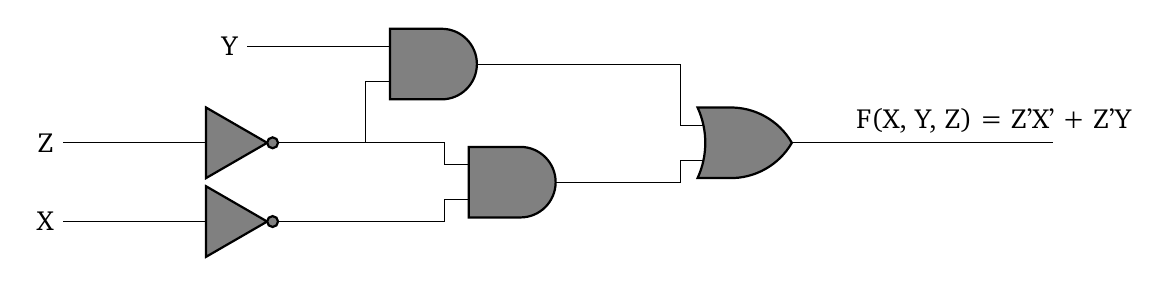
\begin{tikzpicture}
\ctikzset{
    logic ports=ieee,
    logic ports/scale=0.8,
    logic ports/fill=gray
} 
% Logic ports
\node[not port] (nota) at (0,-2){};
\node[not port] (notb) at (0,-3){};
\node[and port] (anda) at (3.5,-2.5){};
\node[and port] (andb) at (2.5,-1){};
\node[or port]  (ora) at (6.5,-2){};
\draw (nota.out) -| (anda.in 1);
\draw (notb.out) -| (anda.in 2);
\draw (anda.out) -| (ora.in 2);
\draw (nota.out) -| (andb.in 2);
\draw (andb.out) -| (ora.in 1);
\draw (ora.out) -- ++(3,0) node[near end,above]{F(X, Y, Z) = Z'X' + Z'Y};
\draw (nota.in 1) -- ++(-1.5,0)node[left]{Z};
\draw (notb.in 1) -- ++(-1.5,0)node[left]{X};
\draw (andb.in 1) -- ++(-1.5,0)node[left]{Y};
\end{tikzpicture}
\end{center}

\subsection{Components}
\begin{table}[!h]
\begin{center}
\begin{tabularx}{0.6\textwidth} { 
  | >{\centering\arraybackslash}X 
  | >{\centering\arraybackslash}X 
  | >{\centering\arraybackslash}X
  | >{\centering\arraybackslash}X | }
\hline
\textbf{Component} & \textbf{Values} & \textbf{Quantity} \\
\hline
Arduino & UNO & 1 \\
\hline
Jumper Wires & M-M & 10 \\
\hline
Breadboard & & 1 \\
\hline
LED & & 2 \\
\hline
Resistor & 220 ohms & 1 \\
\hline
\end{tabularx}
\caption{\label{table:4}List of items required}
\end{center}
\end{table}

\subsection{Implementation and Source Code}
\begin{table}[!h]
\begin{center}
  \begin{tabularx}{0.46\textwidth} { 
  | >{\centering\arraybackslash}X 
  | >{\centering\arraybackslash}X 
  | >{\centering\arraybackslash}X  | }
\hline
\textbf{Arduino PIN} & \textbf{INPUT} & \textbf{OUTPUT} \\ 
\hline
\textbf 2 & X & \\
\hline
\textbf 3 & Y & \\
\hline
\textbf 4 & Z & \\
\hline
\textbf 13 & & F \\
\hline
\end{tabularx}
\caption{\label{table:5}Connections}
\end{center}
\end{table}

\begin{flushleft}

Procedure:\\
\begin{enumerate}[label=\alph*.,labelindent=\parindent,leftmargin=*]
    \item Connect the circuit as per the above table.
    \vspace{2pt}
    \item Connect the output pin to LED.
    \vspace{2pt}
    \item Connect inputs to Vcc for logic 1, ground for logic 0.
    \vspace{2pt}
    \item Execute the circuit using the below code.
    \\
    \vspace{7pt}
    \begin{tabularx}{0.8\textwidth} { 
    | >{\centering\arraybackslash}X |}
    \hline
    https://github.com/shr-eyas/FWC/blob/main/platformio.cpp\\
    \hline
    \end{tabularx}
    \\
    \vspace{10pt}
    \item Change the values of X, Y, Z in the code and verify the truth table.\\
    
\end{enumerate}
\end{flushleft}

%--------------------------------------------------------------------------
\clearpage
\section{Assembly Programming on ATmega328P}

\subsection{Introduction}
A decade counter was implemented by programming an Arduino using the Assembly language instructions for the ATmega328P. This enables one to know about the microcontroller architecture and assembly language.

\subsection{Working Theory}
In addition to what has been mentioned in Section 1.2, Assembly programming is specific to the microcontroller or microprocessor being used and hence is platform dependent. The assembly instructions are written
in an IDE called Geany. Here the Assembly code targets the ATmega328P microcontroller on the Arduino board.

\subsection{Truth Table}
All the Truth Tables and Boolean Logics are same as mentioned in Section 1.3.

\subsection{Source Codes}
\subsubsection{With Decoder IC 7447}
    \begin{tabularx}{0.8\textwidth} { 
    | >{\centering\arraybackslash}X |}
    \hline
    https://github.com/shr-eyas/FWC/blob/main/Assembly/Decade\%20Counter/with7447.asm\\
    \hline
    \end{tabularx}
\\
\subsubsection{Without Decoder IC 7447}
    \begin{tabularx}{0.8\textwidth} { 
    | >{\centering\arraybackslash}X |}
    \hline
    https://github.com/shr-eyas/FWC/blob/main/Assembly/Decade\%20Counter/without7447.asm\\
    \hline
    \end{tabularx}
\\
\subsubsection{With D-Flip Flops}
    \begin{tabularx}{0.8\textwidth} { 
    | >{\centering\arraybackslash}X |}
    \hline
    https://github.com/shr-eyas/FWC/blob/main/Assembly/Decade\%20Counter/withDFlipFlop.asm\\
    \hline
    \end{tabularx}
\\


%----------------------------------------------------------------------
\clearpage
\section{Boolean Verification in Assembly}

\subsection{Introduction}
\begin{flushleft}
$A = a_{1}a_{0}$ and $B = b_{1}b_{0}$ are two 2-bit unsigned binary numbers. If $F(a_{1},a_{0},b_{1},b_{0})$ is a Boolean function such that $F = 1$ only when $A > B$, and $F = 0$ otherwise, then $F$ can be minimized to the form: \vspace{2pt}\\${a_1}\overline{b}_1 + {a_1}{a_0}\overline{b}_0 + {a_0}\overline{b}_0\overline{b}_1$. \vspace{2pt}\\Objective is to verify this equation on Arduino using Assembly Level Language for programming.
\end{flushleft}

\subsection{Working Theory}
\begin{flushleft}
Using the boolean logic output F can be expressed in terms of the inputs X,Y,Z with the help of the following Karnaugh map.
\\
\end{flushleft}
\begin{center}
\begin{karnaugh-map}[4][4][1][${b_1}{b_0}$][${a_1}{a_0}$]

    \maxterms{0,1,2,3,5,6,7,10,11,15}
    \minterms{4,8,9,12,13,14}

    \implicantedge{12}{12}{14}{14}
    \implicant{9}{12}
    \implicant{4}{12}
\end{karnaugh-map}
\\
\vspace{-10pt}
\begin{flushleft}
Karnaugh map simplification results in ${a_1}\overline{b}_1 + {a_1}{a_0}\overline{b}_0 + {a_0}\overline{b}_0\overline{b}_1$
\end{flushleft}
\end{center}

\subsection{Truth Table}
\begin{table}[!h]
\begin{center}
  \begin{tabularx}{0.46\textwidth} { 
  | >{\centering\arraybackslash}X 
  | >{\centering\arraybackslash}X 
  | >{\centering\arraybackslash}X
  | >{\centering\arraybackslash}X 
  | >{\centering\arraybackslash}X 
  | >{\centering\arraybackslash}X 
  | >{\centering\arraybackslash}X 
  | >{\centering\arraybackslash}X 
  | >{\centering\arraybackslash}X 
  | >{\centering\arraybackslash}X | }
\hline
${a_1}$ & ${a_0}$ & ${b_1}$ & ${b_0}$ &\textbf{F}\\
\hline
0 & 0 & 0 & 0 & 0  \\  
\hline
0 & 0 & 0 & 1 & 0  \\  
\hline
0 & 0 & 1 & 0 & 0  \\  
\hline
0 & 0 & 1 & 1 & 0  \\  
\hline
0 & 1 & 0 & 0 & 1  \\  
\hline
0 & 1 & 0 & 1 & 0  \\  
\hline
0 & 1 & 1 & 0 & 0  \\  
\hline
0 & 1 & 1 & 1 & 0  \\  
\hline
1 & 0 & 0 & 0 & 1  \\  
\hline
1 & 0 & 0 & 1 & 1  \\  
\hline
1 & 0 & 1 & 0 & 0  \\  
\hline
1 & 0 & 1 & 1 & 0  \\  
\hline
1 & 1 & 0 & 0 & 1  \\  
\hline
1 & 1 & 0 & 1 & 1  \\  
\hline
1 & 1 & 1 & 0 & 1  \\  
\hline
1 & 1 & 1 & 1 & 0  \\  
\hline
\end{tabularx} \\
\caption{\label{table:6}Truth table for Boolean function 'F'}
\end{center}
\end{table}

\subsection{Digital Schematic}
\begin{center}
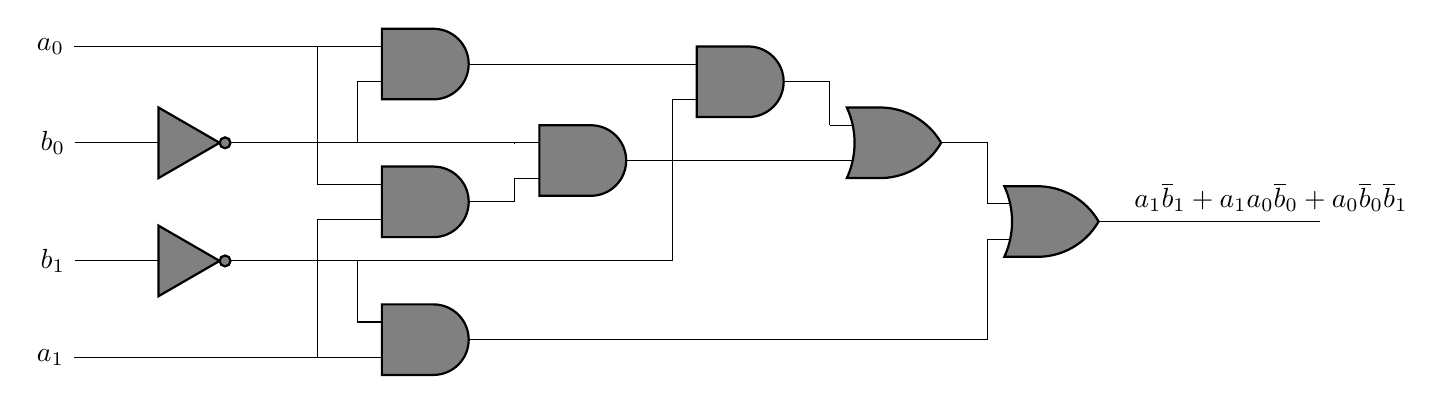
\begin{tikzpicture}
\ctikzset{
    logic ports=ieee,
    logic ports/scale=0.8,
    logic ports/fill=gray
}
% Logic ports
\node[not port] (notb1) at (-1,-3.5){};
\node[not port] (notb0) at (-1,-2){};
\node[and port] (andU) at (2,-1){};
\node[and port] (andM) at (2,-2.75){};
\node[and port] (andD) at (2,-4.5){};
\node[and port] (andX) at (6,-1.225){};
\node[and port] (andY) at (4,-2.225){};
\node[or port]  (orX) at (8,-2){};
\node[or port]  (orY) at (10,-3){};

\draw (notb0.out) -| (andU.in 2);
\draw (notb0.out) -| (andY.in 1);
\draw (notb1.out) -| (andD.in 1);
\draw (notb1.out) -| (andX.in 2);
\draw (andM.out) -| (andY.in 2);
\draw (andU.out) -| (andX.in 1);
\draw (andX.out) -| (orX.in 1);
\draw (andY.out) -| (orX.in 2);
\draw (andD.out) -| (orY.in 2);
\draw (orX.out) -| (orY.in 1);
\draw (andM.in 1) -| ++(-0.5,0) |- (andU.in 1);
\draw (andM.in 2) -| ++(-0.5,0) |- (andD.in 2);
\draw (orY.out) -- ++(2.5,0) node[near end,above]{${a_1}\overline{b}_1 + {a_1}{a_0}\overline{b}_0 + {a_0}\overline{b}_0\overline{b}_1$};
\draw (andU.in 1) -- ++(-3.6,0)node[left]{${a_0}$};
\draw (andD.in 2) -- ++(-3.6,0)node[left]{${a_1}$};
\draw (notb1.in 1) -- ++(-0.75,0)node[left]{${b_1}$};
\draw (notb0.in 1) -- ++(-0.75,0)node[left]{${b_0}$};
\end{tikzpicture}
\end{center}

\subsection{Components}
\begin{center}
\begin{table}[!h]
\centering
\begin{tabularx}{0.6\textwidth} { 
  | >{\centering\arraybackslash}X 
  | >{\centering\arraybackslash}X 
  | >{\centering\arraybackslash}X
  | >{\centering\arraybackslash}X | }
\hline
\textbf{Component} & \textbf{Values} & \textbf{Quantity} \\
\hline
Arduino & UNO & 1 \\
\hline
Jumper Wires & M-M & 10 \\
\hline
Breadboard & & 1 \\
\hline
LED & & 2 \\
\hline
Resistor & 220 ohms & 1 \\
\hline
\end{tabularx}
\caption{\label{table:7}List of items required}
\centering
\end{table}
\end{center}

\subsection{Implementation and Source Code}
\begin{table}[!h]
\begin{center}
  \begin{tabularx}{0.46\textwidth} { 
  | >{\centering\arraybackslash}X 
  | >{\centering\arraybackslash}X 
  | >{\centering\arraybackslash}X  | }
\hline
\textbf{Arduino PIN} & \textbf{INPUT} & \textbf{OUTPUT} \\ 
\hline
\textbf 2 & a0 & \\
\hline
\textbf 3 & a1 & \\
\hline
\textbf 4 & b0 & \\
\hline
\textbf 5 & b1 & \\
\hline
\textbf 8 & & F \\
\hline
\end{tabularx}
\caption{\label{table:8}Connections}
\end{center}
\end{table}

\begin{flushleft}

Procedure:\\
\begin{enumerate}[label=\alph*.,labelindent=\parindent,leftmargin=*]
    \item Connect the circuit as per the above table.
    \vspace{2pt}
    \item Connect the output pin to LED.
    \vspace{2pt}
    \item Connect inputs to Vcc for logic 1, ground for logic 0.
    \vspace{2pt}
    \item Execute the circuit using the below code.
    \\
    \vspace{7pt}
    \begin{tabularx}{0.8\textwidth} { 
    | >{\centering\arraybackslash}X |}
    \hline
    https://github.com/shr-eyas/FWC/blob/main/Assembly/assembly.asm\\
    \hline
    \end{tabularx}
    \\
    \vspace{10pt}
    \item Change the values of X, Y, Z in the code and verify the truth table.\\
    
\end{enumerate}
\end{flushleft}

%----------------------------------------------------------------------------------------------
\clearpage
\section{Embedded C and AVR-GCC}

\subsection{Introduction}
\justifying
AVR-GCC, in particular, is a version of GCC optimized for compiling C and C++ code for AVR microcontrollers.\\
Objective here is to verify the correct operation of a divide-by-5 counter implemented using a 7474 IC where the binary count is displayed using seven segment display. The program for verification must be written in Embedded C and compiled using AVR-GCC.\\


\subsection{Components}
\begin{table}[!h]
\begin{center}
\begin{tabularx}{0.6\textwidth} { 
  | >{\centering\arraybackslash}X 
  | >{\centering\arraybackslash}X 
  | >{\centering\arraybackslash}X
  | >{\centering\arraybackslash}X | }
\hline
\textbf{Component} & \textbf{Values} & \textbf{Quantity} \\
\hline
Arduino & UNO & 1 \\
\hline
Jumper Wires & M-M & 30 \\
\hline
Breadboard & & 1 \\
\hline
Seven Segment Display & Common Anode & 1 \\
\hline
Resistor & 220 ohms & 1 \\
\hline
IC & 7474 & 2 \\
\hline
IC & 7447 & 1 \\
\hline
\end{tabularx}
\caption{\label{table:9}List of items required}
\end{center}
\end{table}

\subsection{Digital Schematic}
\begin{center}
\begin{figure}[htbp]
        \centering
        \includegraphics[scale = 0.8]{1.png}
\end{figure}  
\end{center}

\subsubsection{Boolean Equation}
From the circuit diagram we can conclude:
\begin{align}
    D0 &=\overline{ (Q1 + Q2) }\\
    D1 &= Q0\\
    D2 &= Q1
\end{align}
\vspace{5pt}

\subsection{Truth Table}
\begin{center}
\begin{table}[!h]
\centering
  \begin{tabularx}{0.6\textwidth} { 
  | >{\centering\arraybackslash}X 
  | >{\centering\arraybackslash}X 
  | >{\centering\arraybackslash}X
  | >{\centering\arraybackslash}X 
  | >{\centering\arraybackslash}X 
  | >{\centering\arraybackslash}X 
  | >{\centering\arraybackslash}X 
  | >{\centering\arraybackslash}X 
  | >{\centering\arraybackslash}X 
  | >{\centering\arraybackslash}X | }
\hline
\textbf{Q2} & \textbf{Q1} & \textbf{Q0} & \textbf{D2} & \textbf{D1} & \textbf{D0} & \textbf{Q2'} & \textbf{Q1'} & \textbf{Q0'}\\
\hline
0 & 0 & 0 & 0 & 0 & 1 & 0 & 0 & 1 \\  
\hline
0 & 0 & 1 & 0 & 1 & 1 & 0 & 1 & 1 \\  
\hline
0 & 1 & 1 & 1 & 1 & 0 & 1 & 1 & 0 \\  
\hline
1 & 1 & 0 & 1 & 0 & 0 & 1 & 0 & 0 \\  
\hline
1 & 0 & 0 & 0 & 0 & 0 & 0 & 0 & 0 \\  
\hline
\end{tabularx} \\
\caption{\label{table:10}Truth table for the given circuit}
\centering
\end{table}
\end{center}

\subsection{Implementation and Source Code}
\vspace{10pt}
\begin{enumerate}[label=\alph*.,labelindent=\parindent,leftmargin=*]

    \item Make the connections between the seven segment display and the 7447 IC as shown below. 
    \begin{table}[htbp]
      \centering
      \begin{tabular}{|>{\centering\arraybackslash}m{2cm}|*{7}{>{\centering\arraybackslash}m{1cm}|}}
        \hline
        7447 & $\overline{a}$ & $\overline{b}$ & $\overline{c}$ & $\overline{d}$ & $\overline{e}$ & $\overline{f}$ & $\overline{g}$ \\
        \hline
        Display & a & b & c & d & e & f & g \\
        \hline
      \end{tabular}
      \label{tab:sample}
    \end{table}

    \item Connect the Arduino, 7447 and the two 7474 ICs according to below table.
    \begin{table}[htbp]
      \centering
      \begin{tabular}{|c|c|c|c|c|c|c|c|c|c|c|c|c|}
        \hline
        \multirow{2}{*}{} & \multicolumn{3}{c|}{INPUT} & \multicolumn{3}{c|}{OUTPUT} & \multicolumn{2}{c|}{CLOCK} & \multicolumn{4}{c|}{5V}\\
        \cline{2-7}
         & Q0 & Q1 & Q2 & Q0' & Q1' & Q2' & \multicolumn{2}{c|}{} & \multicolumn{4}{c|}{} \\
        \hline        
        Arduino & D6 & D7 & D8 & D2 & D3 & D4 & \multicolumn{2}{c|}{D13} & \multicolumn{4}{c|}{}\\
        \hline
        7474 & 5 & 9 & {} & 2 & 12 & {} & CLK1 & CLK2 & 1 & 4 & 10 & 13\\
        \hline
        7474 & {} & {} & 5 & {} & {} & 2 & CLK1 & CLK2 & 1 & 4 & 10 & 13\\
        \hline
        7447 & \multicolumn{3}{c|}{} & 7 & 1 & 2 & & & \multicolumn{4}{c|}{16}\\
        \hline 
      \end{tabular}
      \label{tab:merge-cells}
    \end{table}

    \item Hence we have implemented the divide by 5 counter digital circuit. Execute the circuit using below code. \vspace{10pt} \\
    \begin{tabularx}{0.8\textwidth} { 
    | >{\centering\arraybackslash}X |}
    \hline
    https://github.com/shr-eyas/FWC/blob/main/Embedded\%20C/counter.c\\
    \hline
    \end{tabularx} \\
\end{enumerate}

%--------------------------------------------------------------------------------
\clearpage
\section{Project 1}

\subsection{Introduction}
\begin{flushleft}
This main objective of this project is to make an unmanned ground vehicle (UGV) follow an exact straight path which it naturally does not do because of unavoidable mechanical errors.
\end{flushleft}

\subsection{Working Theory}
\begin{flushleft}
\justifying
To achieve the objective, a simple technique known as differential drive control is used. Encoders attached to the wheels will count the number of rotations and hence distance traveled by each wheel. Further, a closed loop control system directs the wheel to control its rotation speed on basis of the error measured. Error here is the difference between number of rotations of each wheel. Ideally, both the wheels must rotate by equal amounts to make the UGV go straight. 
\end{flushleft}

\subsection{Components}
\begin{table}[!h]
\begin{center}
\begin{tabularx}{0.6\textwidth} { 
  | >{\centering\arraybackslash}X 
  | >{\centering\arraybackslash}X 
  | >{\centering\arraybackslash}X
  | >{\centering\arraybackslash}X | }
\hline
\textbf{Component} & \textbf{Values} & \textbf{Quantity} \\
\hline
ESP & 32 & 1 \\
\hline
Motor Driver & L293D & 1 \\
\hline
DC Motor & 7.4V & 2 \\
\hline
UGV Chassis & & 1 \\
\hline
Breadboard & & 1 \\
\hline
Encoder & Optical & 2 \\
\hline
Jumper Wires & M-M & 10 \\
\hline
Jumper Wires & M-F & 10 \\
\hline
LiPo Battery & 7.4V & 1 \\
\hline
\end{tabularx}
\caption{\label{table:4}List of items required}
\end{center}
\end{table}

\subsection{Digital Schematic}
\begin{center}
\begin{figure}[htbp]
        \centering
        \includegraphics[scale = 0.5]{3.png}
\end{figure}  
\end{center}


\subsection{Implementation and Source Code}
\vspace{10pt}
\begin{enumerate}[label=\alph*.,labelindent=\parindent,leftmargin=*]

    \item Assemble the UGV Chassis, make the connections as per the wiring diagram and put both the systems together.

    \item Upload the following code on ESP32. This code has no closed control loop and just provides both motors with equal power. \vspace{10pt} \\
    \begin{tabularx}{0.9\textwidth} { 
    | >{\centering\arraybackslash}X |}
    \hline
    https://github.com/shr-eyas/Robotics/blob/main/IIT\%20Hyderabad\%20/UGV/noLoopUGV.cpp\\
    \hline
    \end{tabularx} \\

    \item Now put the UGV on the floor with no obstacles in the way and then plug in the battery.

    \item The UGV deviates instead of going exactly straight. This deviation is easily visible as it mostly ends up going in a curved path.  

    \item Following this, re-upload the following code on ESP32. This code has a closed control loop which will make the UGV follow the path of a straight line. \vspace{10pt} \\
    \begin{tabularx}{0.9\textwidth} { 
    | >{\centering\arraybackslash}X |}
    \hline
    https://github.com/shr-eyas/Robotics/blob/main/IIT\%20Hyderabad\%20/UGV/pdUGV.cpp\\
    \hline
    \end{tabularx} \\

    \item Now once again put the UGV on the floor with no obstacles in the way and then plug in the battery.

    \item This time, it can be seen that the UGV follows a straight line path instead of going on a curved trajectory.
    
\end{enumerate}



%--------------------------------------------------------------------------------
\clearpage
\section{Project 2}

\subsection{Introduction}
\begin{flushleft}
This main objective of this project is to demonstrate the use of machine learning in beacon tracking using an unmanned ground vehicle (UGV) and a WiFi-enabled microcontroller such as the ESP32.
\end{flushleft}

\subsection{Working Theory}
\begin{flushleft}
\justifying
Initially, the ESP32 mounted on the car reads the RSSI (Radio Signal Strength Indicator) levels in the forward, right, and left directions through suitable in-place rotation. To ensure accurate RSSI readings, an average of 20 RSSI values is taken for each direction. Subsequently, the car rotates towards the direction with the highest RSSI level, indicating the strongest signal from the beacon. It then proceeds to move forward continuously in that direction, maintaining alignment with the beacon's signal. By repeating above steps again and again, the car navigates towards the beacon.
\end{flushleft}

\subsection{Components}
\begin{table}[!h]
\begin{center}
\begin{tabularx}{0.6\textwidth} { 
  | >{\centering\arraybackslash}X 
  | >{\centering\arraybackslash}X 
  | >{\centering\arraybackslash}X
  | >{\centering\arraybackslash}X | }
\hline
\textbf{Component} & \textbf{Values} & \textbf{Quantity} \\
\hline
ESP & 32 & 1 \\
\hline
Motor Driver & L293D & 1 \\
\hline
DC Motor & 7.4V & 2 \\
\hline
UGV Chassis & & 1 \\
\hline
Breadboard & & 1 \\
\hline
Jumper Wires & M-M & 10 \\
\hline
Jumper Wires & M-F & 10 \\
\hline
LiPo Battery & 7.4V & 1 \\
\hline
\end{tabularx}
\caption{\label{table:4}List of items required}
\end{center}
\end{table}

\subsection{Digital Schematic}
\begin{figure}[htbp]
        \begin{center}
        \includegraphics[scale = 0.5]{3.png}    
        \end{center}
\end{figure}   

\subsection{Implementation and Source Code}
\vspace{10pt}
\begin{enumerate}[label=\alph*.,labelindent=\parindent,leftmargin=*]

    \item Assemble the UGV Chassis, make the connections as per the wiring diagram and put both the systems together.
    
    \item Upload the following code on ESP32. \vspace{10pt} \\
    \begin{tabularx}{0.9\textwidth} { 
    | >{\centering\arraybackslash}X |}
    \hline
    https://github.com/shr-eyas/Robotics/blob/main/IIT\%20Hyderabad\%20/Beacon\%20Tracking/beacon.cpp\\
    \hline
    \end{tabularx} \\

    \item Now put the phone at a reasonable distance from the UGV with no obstacles in the way and then turn on the hotspot. The UGV should travel towards the phone and stop near it.

    \item The algorithm described above is very basic and crude way to navigate toward the beacon. Frequent left and right rotation is required to identity the direction having the maximum RSSI level.

    \item Using this algorithm, only 60-70 percent of the time (i.e. 60-70\% Accuracy), the car rotates and moves towards the correct direction. Due to low accuracy, The car may take time to reach till the beacon.
\end{enumerate}


\end{document}
